\begin{figure}[h!]
	\centering
	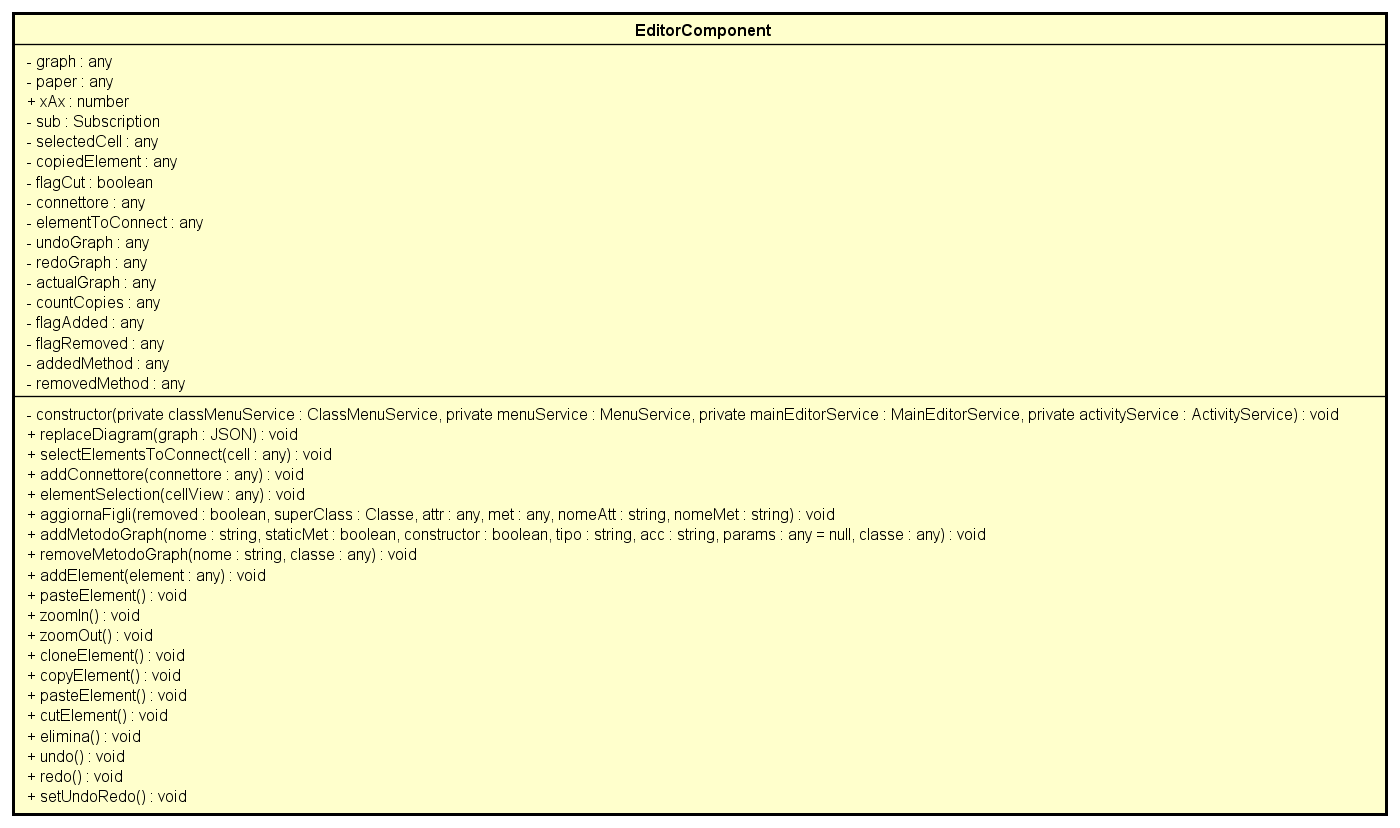
\includegraphics[scale=0.8]{res/sections/SpecificaFrontEnd/Components/Disegnetti/editor.png}
	\caption{Diagramma della classe EditorComponent}
\end{figure}

\begin{itemize}
	\item \textbf{Descrizione:}\\
	
	\item \textbf{Utilizzo:}\\
	
	\item \textbf{Attributi:}
		\begin{itemize}
			\item \emph{-graph: any}\\
            Contiene tutti gli elementi del grafico
            \item \emph{-paper: any}\\
            Assicura che vengano renderizzati gli elementi del grafico
            \item \emph{+xAx: number}\\
            Serve per scalare il grafico
            \item \emph{-sub: Subscription}\\
            Permette la funzione di zoom
            \item \emph{-selectedCell: any}\\
            Punta all'elemento selezionato con il click
            \item \emph{-copiedElement: any}\\
			Punta all'elemento copiato o tagliato
			\item \emph{-flagCut: boolean}\\
			Indica se l'elemento è stato tagliato, altrimenti è stato copiato
            \item \emph{-connettore: any}\\
            Il tipo del connettore selezionato
            \item \emph{-elementToConnect: any}\\
            Punta all'elemento selezionato con il click, che sarà collegato con il connettore
			\item \emph{-undoGraph: any}\\
			Punta al grafico dopo aver annullato l'ultima operazione
			\item \emph{-redoGraph: any}\\
			Punta al grafico dopo aver ripristinato l'ultima operazione annullata
			\item \emph{-actualGraph: any}\\
			Punta al grafico attuale
			\item \emph{-countCopies: any}\\
			Conta il numero di copie dello stesso elemento
			\item \emph{-flagAdded: any}\\
			Indica se bisogna ascoltare l'evento aggiungere del grafo
			\item \emph{-flagRemoved:any}\\
			Indica se bisogna ascoltare l'evento rimuovere del grafo
			\item \emph{-addedMethod: any}\\
			Indica al metodo annulla se un metodo è stato aggiunto
			\item \emph{-removedMethod: any}\\
			Indica al metodo annulla se un metodo è stato rimosso
		\end{itemize}
	\item \textbf{Metodi:}
		\begin{itemize}
			\item \emph{}\\
    		\\
    		\textbf{Parametri:}
    		\begin{itemize}
    			\item \emph{}\\
    			
    		\end{itemize}
		\end{itemize}
\end{itemize}